
\chapter{Measurement, Uncertainty, and Temperature}

%%%%%%%%%%%%%%%%%%%%%%%%%%%%%%%%%%%%%%%%%%%%%
\section*{Equipment List}

\begin{multicols}{2}   % change 2 -> 3 for three columns
\begin{equipment}
  \item Leslie Cube
  \item Glass Thermometer
  \item IR Thermometer ``gun'' (2)
  \item Stopwatch
  \item Ruler
  \item Computer
\end{equipment}
\end{multicols}

%%%%%%%%%%%%%%%%%%%%%%%%%%%%%%%%%%%%%%%%%%%%%
\section*{Overview}

In this weekly lab you will primarly work in pairs, with your ``partner'' at the same table, but feel free to discuss things with the ``group'' of four at your adjoining tables.  We will also share data with the entire class, usually using google surveys and sheets.  You will turn in your own individual lab assignment, with copies of all data and graphs, in a single pdf document uploaded to the Blackboard ``assignment'' for that week.

%%%%%%%%%%%%%%%%%%%%%%%%%%%%%%%%%%%%%%%%%%%%%
\section{Introduction and Definitions}

Today we will conduct our first measurements of physical phenomena, mostly temperature measurements, and understand the necessity of the uncertainty and units associated with those measurements.
	%
	\begin{itemize} 
	\item[] A \defterm{physical measurement} contains three equally important parts: the numerical \defterm{value}, the \defterm{uncertainty} (also referred to as {\em error}) in that value, and the \defterm{units} in which these are measured.
	\end{itemize}
	%
Some examples are:
	%
	\begin{itemize}
	\item[-] The human body temperature is $37.0 \pm 0.5$ $\degree$C.\\
	{\small (Uncertainty represented as ``plus or minus'' makes a range of values. Both the value and uncertainty are in ``degrees celsius''.)}
	\item[-] A college basketball game has 40~minutes $\pm 0.1$~seconds of playing time.\\
	{\small (The final minute clock measures to tenths of a second. The units can be different between the value and uncertainty.}
	\item[-] The Sun is 93 million miles away\\
	{\small Here the uncertainty is expressed {\em implicitly} as ``plus or minus a few of the last digit given'', so plus or minus a few million miles}
	\end{itemize}
	%
Let's make a precise definition of the uncertainty/error in a measurement:
	%
	\begin{itemize}
	\item[] Given a particular measurement, the \defterm{uncertainty} is a statement of the range of values in which another scientist is likely\footnote{More precisely, if we say that the uncertainty is the {\em standard deviation} over repeated measurements, then 68\% of all measurements fall in that range} to make the same measurement.
	\end{itemize}
	%
There are a number of sources/components of this uncertainty:
	%
	\begin{itemize}
	\item[-] \defterm{Instrumental Uncertainty}: A measurement device generally has a smallest unit division shown. For an analog device --- like a ruler with millimeter marks, or a thermometer with degrees --- where we might hope to measure between the smallest markings, we can specify the instrumental uncertainty as such (e.g., half of a millimeter on a ruler, or 0.3$\degree$C on a thermometer).  For a digital device, we can say that the instrumental uncertainty is ``plus or minus a few of the last digit'' (e.g., $\pm 0.03$~seconds on a standard stopwatch).  
	\item[-]  \defterm{(Manufacturing) Instrumental Uncertainty}: Sometimes although an instrument shows a precise demarcation, it is clear from looking at multiple ``identical'' instruments that they were not manufactured to that precision (e.g., multiple identical thermometers read slightly different values).  The range of manufacturing uncertainty can be assessed by using multiple copies of the same device.
	\item[-] \defterm{Methodological Uncertainty}: Sometimes our uncertainty is limited more by the way we make a measurement than by the instrument itself.  For example, although a stopwatch has instrumental uncertainty in the hundreths of a second, our human reaction time is no better than a few {\em tenths} of a second, so our methodological uncertainty would be $\pm0.3$~s.  This can be assessed by making repeated measurements.
	\item[-] \defterm{Natural Variation} Almost always, the object of measurement does not have an infinitely precise value (e.g., the ``temperature outside right now'' depends on where exactly you measure it, and at which moment in time; the ``diameter of a rock'' that is not spherical).  This uncertainty can sometimes be limited by a more precise specification of the measurement (e.g., ``the temperature in the shade, outside Padnos, at 10:40 am''; or ``the largest diameter of the rock'').  And, like the methodological uncertainty, it can be assessed by repeated measurements.
	\end{itemize}
	%
	
	
%%%%%%%%%%%%%%%%%%%%%%%%%%%%%%%%%%%%%%%%%%%%%
\section{Experiments}

%%%%%%%%%%%%%%%%%%%%%%%%%%%%%%%%%%
\subsection{The time of my name}

\begin{itemize}
\item Have your partner recite their full name to you at a steady relaxed pace.  Measure the amount of time this takes using the stopwatch.  You can try this multiple times.  Then switch and recite your own name for them.
\end{itemize}
%
\subsubsection*{Questions}
\begin{questions}
\Q{Write down the name, and then your time measurement with uncertainty and units.}
\Q[6\baselineskip]{Briefly explain how you arrived at the uncertainty value, making mention of all ``sources'' of uncertainty.}
\end{questions}



%%%%%%%%%%%%%%%%%%%%%%%%%%%%%%%%%%
\subsection{``Seeing'' the uncertainty I: Room Temperature}

One table has been set up with an array of thermometers.  Since they are all localized in the same place, they should be making approximately the same measurement: the temperature of the air at that table right now.
	%
	\begin{itemize}
	\item Take a careful clear photo of the array of thermometers, then return to your desk and write down each of the temperature measurements on a sheet of paper.
	\item Considering the range of measurements you have, put labeled tick marks \underline{on the axis below} such that the values will be spread out across the line. Use a ruler to make equal spacing of tick marks.  At the far right, label that axis (e.g., ``Temperature (C)'').
	\item Place a dot on/near the axis for every measurement of temperature.  You can ``scatter'' these a bit above/below the axis for clarity.
	\end{itemize}
	%
%%%%%%% BEGIN FIGURE %%%%%%%%%
\begin{center}
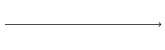
\includegraphics[width=\textwidth]{images/01_axis}
\end{center}
%%%%%%%   END FIGURE   %%%%%%%%%
	%
\subsubsection*{Questions}
\begin{questions}
\Q{Express the full measurement with value, uncertainty, units. Estimate the uncertainty using your graphical display of points.}
\Q{What is the instrumental uncertainty for this thermometer?}
\Q[8\baselineskip]{What do you think is the primary source of the uncertainty?  Mention each type of uncertainty source.}
\end{questions}


%%%%%%%%%%%%%%%%%%%%%%%%%%%%%%%%%%
\subsection{``Seeing'' the uncertainty II: Body Temperature}

Here each of you will make a measurement of your body temperature using the Infrared (IR) thermometer ``gun'' on the palm of your hand.  Note the picture on the side of the IR thermometer gun describing its ``beam'' of measurement (imagine a spot being projected onto the thing you are measuring, and make sure the spot is contained within the object).  You will produce a two-picture plot, using a provided code (see Blackboard) and the Google CoLab implementation of python programming language.
%
\begin{questions}
\Q{What is the instrumental uncertainty associated to the IR thermometer?}
\Q{Do you observe any natural variation of temperature across your hand?}
\Q{Write down your measurement (with value, uncertainty, and units) here, and then submit it to the google survey (see Blackboard).}
\end{questions}
%
\begin{itemize}
\item Copy the column of ``values'' data for the whole class in the linked spreadsheet (see Blackboard) into your own spreadsheet and save as a csv file.
\item In a web browser, go to \verb|colab.research.google.com| and open a ``New Notebook''.
\item Paste in the code provided on blackboard for {\em Scatter and Histogram Plot}.
\item To run the code, either press the ``play'' button, or press shift-enter/shift-return.  It will prompt you for your csv file to upload.
\item This will produce a plot on the screen.
\item Notice that there are generic axis labels and titles.  Find the place in the code where they have been entered and edit them to make them specific to your particular data.
\item To save and print your plot, you can either right-click and save to a file or screenshot to a file.  Print this plot so that you can add it to your submission.
\end{itemize}

%%%%%%%%%%%%%%%%%%%%%%%%%%%%%%%%%%
\subsection{Leslie Cube}

\begin{itemize}
\item Fill up the Leslie cube with hot/warm water at the sink and then replace the rubber stopper. Fill a small beaker with cold water.
\item Place the glass thermometer first in the cold water, and then insert it into the Leslie cube such that its bulb is in the middle of the cube.
\end{itemize}
%
\begin{questions}
\Q{Record the glass thermometer measurements of the temperature in the cold water and in the Leslie cube.}
\Q{Describe how quickly the thermometer came to equilibrium with the cold water and with the hot water.}
\Q{Take and record temperature measurements of \underline{each side} of the Leslie cube using the IR thermometer gun.}
\end{questions}


%%%%%%%%%%%%%%%%%%%%%%%%%%%%%%%%%%
\subsection{Temperatures of other objects}

\begin{itemize}
\item Using the IR thermometer gun, record measurements of temperature (with value, uncertainty, units for each) for some of the following objects:
	%
	\begin{itemize}
	\item The surface of the table you sitting at.
	\item Something else in the room.
	\item Outside: Something that might be in equilibrium with the air temperature (shaded spot).
	\item Outside: Something that is probably not in equilibrium with the air temperature.
	\item Outside: The sky (try both clear and clouded spots).
	\end{itemize}
\item Record your temperature measurements below and also report them to the google survey posted on Blackboard.
\end{itemize}

\begin{questions}
\Q[16\baselineskip]{Record your temperature measurements here.}
\end{questions}


%- ``diameter'' of a rock
%- IR gun on difffernet parts of table
%- width of a cloud?
%
%What is ``human error''?
%
%Definition Temperature, Temperature scales
%
%Measure temperature of water in leslie cube (preped with some amount of boiling water within room temp)
%- glass thermometer best measure (talk about why)
%- observe how quickly it comes to equilibrium (measure with stopwatch, cell phone)
%- now IR thermometer as directed at water, and each side
%
%How does IR thermometer work, how do we account for various surfaces
%
%Uncertainty due to ``bias'' ... temperature of water and leslie cube all same, but IR gun gives sign diff values.  What are they, how do we account/correct for it?
%
%
%Temperature of outside (IR gun)
%- air temperature (I place a themometer outside) ... how long does it take glass thermometer to reach equilibrium?
%- ground, trees, buildings, sidewalks etc
%- sky (variation in location on sky, clear vs clouds...?)
%
%Collect data and use google colab to plot
%- python script for histograms , plot
%- python script for scatter, plot
%- 
%
%Instructions for next week: collect temperature data from your location, upload to google sheet

%%%%%%%%%%%%%%%%%%%%%%%%%%%%%%%%%%
\subsection*{Summary Questions}

Brief answers are fine, but please write in complete sentences.

\begin{questions}
\Q{State the temperature measurements you made for the Leslie cube, including each type of side and the direct glass thermometer measurement.  Speculate on why you found different values, if you did.}
\Q[8\baselineskip]{Looking at either the hand-temperature data or the other plot you made with the entire class data: how did your own estimated uncertainty (for your measured value) compare to the ``spread'' of the data taken by all students?  Should these agree?  Why or why not?}
\Q{Two students make a measurement of the distance from the Bookstore to the Clock Tower.  They are reported as follows
%
\begin{equation*}
\begin{split}
\unit{199.65}{\meter} & \pm \unit{0.3}{\meter}\\
\unit{202}{\meter} & \pm \unit{3}{\meter}
\end{split}
\end{equation*}
%
(i) On the axis below, draw tick marks over a wide enough range to plot both measurements {\em and their ranges of uncertainty}.  (ii) Plot the two measurements using a point for the ``value'' and a horizontal bar to show the uncertainty. (iii)Are these ``the same'' measurements to within uncertainty or not?  Explain.}
\Q{Shown below is a summary of the Global Average Temperature over most of human recorded history.  The uncertainties for each data point are indicated by bars. Speculate on how these uncertainties might have been determined, how they change over time, and why.}
\end{questions}


	%
%%%%%%% BEGIN FIGURE %%%%%%%%%
\begin{center}
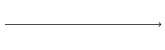
\includegraphics[width=\textwidth]{images/01_axis}
\end{center}
%%%%%%%   END FIGURE   %%%%%%%%%
	%
	
	
	%
%%%%%%% BEGIN FIGURE %%%%%%%%%
\begin{center}
\includegraphics[width=0.75\textwidth]{images/01_global-avg-temperature-1860-present_may-2025-report_BEST.png}
\end{center}
%%%%%%%   END FIGURE   %%%%%%%%%
	%
